%% Font size %%
\documentclass[11pt]{article}

%% Load the custom package
\usepackage{Mathdoc}

%% Numéro de séquence %% Titre de la séquence %%
\renewcommand{\centerhead}{Devoir  \#1 : Divisions Euclidiennes}

%% Spacing commands %%
\renewcommand{\baselinestretch}{1} \setlength{\parindent}{0pt}


\begin{document}

\entetedevoirs{30}

\begin{center}
\duree{55 minutes} 
\coefficient{1}
\calculatrice{0}
\brouillon
\copieseparee{0}
\end{center}

\begin{multicols}{2}
\begin{exercicedevoir}[5][Compléter les égalités]
\begin{multicols}{2}
\begin{enumerate}
\item $6\times \ldots\ldots =48$
\item $7\times \ldots\ldots =49$
\item $ \ldots\ldots \times 9 =36$
\item $5\times \ldots\ldots =15$
\item $ \ldots\ldots \times 5 =30$
\item $ \ldots\ldots \times 4 =28$
\item $5\times \ldots\ldots =30$
\item $4\times \ldots\ldots =32$
\item $7\times \ldots\ldots =63$
\item $ \ldots\ldots \times 7 =28$
\end{enumerate}
\end{multicols}
\end{exercicedevoir}

\begin{exercicedevoir}[5][Compléter le tableau]
\renewcommand{\arraystretch}{1.5}
\begin{tabular}{|c|c|c|}
\hline
Diviser & Quotient & \phm Reste \phm \\ \hline
43 par 6&7&1\\ \hline
46 par 5&&\\ \hline
22 par 4&&\\ \hline
26 par 3&&\\ \hline
39 par 6&&\\ \hline
47 par 8&&\\ \hline
\end{tabular}
\end{exercicedevoir}
\end{multicols}

\begin{exercicedevoir}[8][Compléter les divisions suivantes]
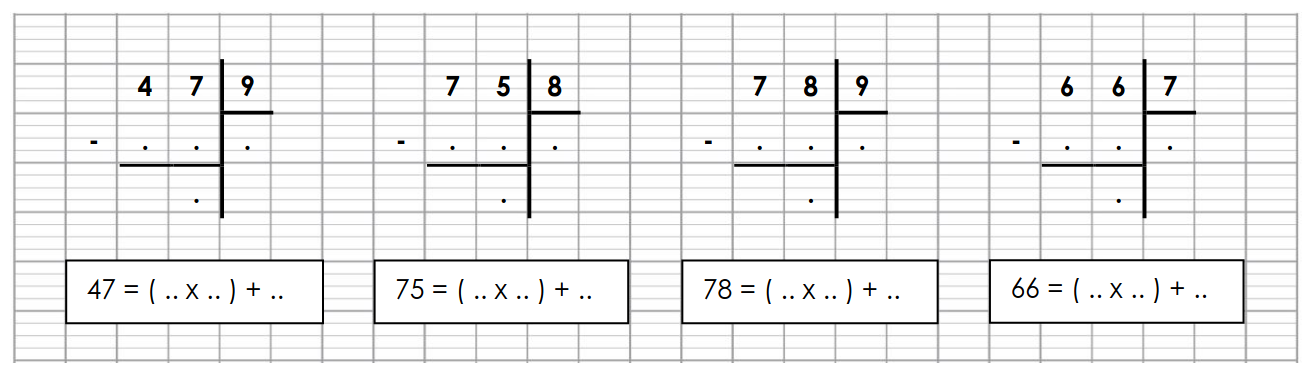
\includegraphics[width=\linewidth]{.data/DIVISION-1.png}
\end{exercicedevoir}

\begin{exercicedevoir}[8][Compléter les divisions suivantes]
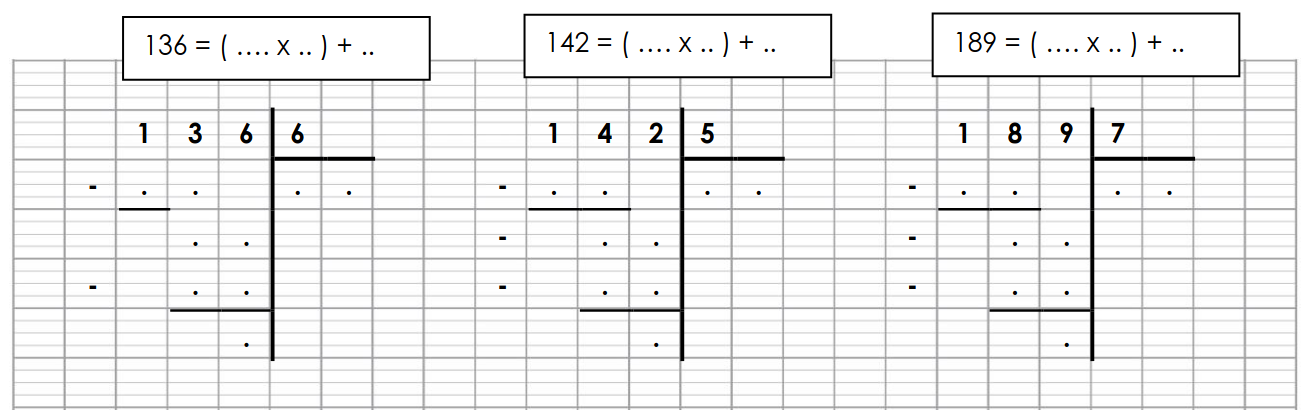
\includegraphics[width=\linewidth]{.data/DIVISION-2.png}
\end{exercicedevoir}

\begin{exercicedevoir}[4][Résolution de problème I]
Une fleuriste désire faire des bouquets de 5 roses avec les 48 fleurs qu’elle
possède. \\
Combien de bouquets pourra-t-elle faire et combien de fleurs lui
restera-t-il ?
\end{exercicedevoir}
\encart{5cm}

\begin{exercicedevoir}[4][Résolution de problème II]
Julie lit chaque soir 9 pages de son roman qui en compte 135.\\
Combien de jours mettra-t-elle pour finir son livre ?
\end{exercicedevoir}
\encart{5cm}

\end{document}

%%% Local Variables:
%%% mode: LaTeX
%%% TeX-master: t
%%% TeX-master: t
%%% gptel-model: deepseek-chat
%%% gptel--backend-name: "DeepSeek"
%%% gptel--bounds: ((998 . 1031) (1346 . 1402) (1486 . 1542))
%%% End:

